%%%%%%%%%%%%%%%%%%%%%%% 需求分析 %%%%%%%%%%%%%%%%%%%%%%%%%%%%%%%%%%%%%%%%%%
\chapter{需求分析}

\label{cha:demand_analysis}
\section{问题陈述}


我国海鲜市场的体量因巨大的人口基数的存在,也是十分庞大,随着近年来社会经济的进一步发展,市场对海鲜的需求量也在进一步上升,但是由于现阶段市场缺乏买卖双方稳定、高效且低成本的沟通机制,海鲜从生产到上市中间的资料消耗往往占了成本的很大一部分。因此我们分析并实现一个连接微供应商和订购商之间的一个中间平台“鲜天下”。通过该平台,我们得以更好的利用目前现存而又无法替代的小作坊,从而聚合微供应商的生产力,满足大厂家的订单需求,同时确保大订购商稳定的供应来源以及降低大订购商与小作坊的沟通成本。

本平台主要客户为养虾户(以下称为微供应商)以及对虾有较大需求的厂家(以下称为订购商)。微供应商和订购商需要在该系统上进行注册并等待管理员认证,若认证成功,订购商可通过该平台发起订单,并实时查看该订单的提交情况与完成情况,如果订单被平台所接受并完成,订购商需要向平台支付款项。

微供应商可以在“鲜天下”平台上注册申请成为认证微供应商,并能够查看目前平台上由订购商发布的母订单。在母订单列表中,微供应商能够从中选择并加入列表中的订单,按时交付,同时完成订单后还能够从平台中得到相应款项。


为确保微供应商与订购商之间的协作安全,平台管理人员会对平台所接收到的来自订购商的订单进行审核,并确定是否存在无效订单,由此,管理人员可根据需要取消某些不合法的订单。管理人员还能够对平台目前的订单以及用户进行相关的处理,如对部分用户进行封禁,关闭某些正在进行中的订单等。


该平台采用微服务架构,前端、后端还有数据库分别使用docker封装,通过将应用和服务分解成更小的、松散耦合的组件,它们可以更加容易升级和扩展,并以可独立部署的服务套件发布,用户可根据成本以及性能要求将这些服务部署在一台服务器上或者分别部署在不同的服务器中。


\section{用例析取}

对“鲜天下”平台,我们完成了用例图,图示见\autoref{fig:usecase-main}\footnote{“鲜天下”系统分析于设计中所有的UML制品均由PlantUML开源项目生成,遵循最新的uml2.0规范。}。

%\usepackage{changepage}
%\usepackage{rotating}
%\usepackage{float}
%\usepackage[section]{placeins}
%\begin{sidewaystable}[!Htp]
\begin{figure}[htp]
    %\begin{adjustwidth}{-1.5cm}{-1cm}
    \centering
    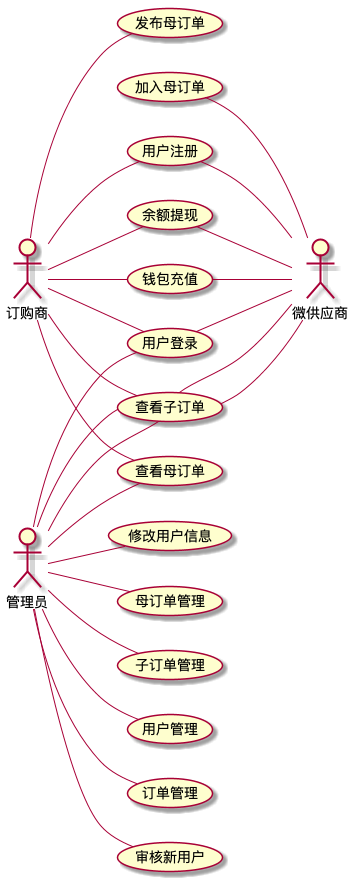
\includegraphics[width=8cm]{report/figure/usecase/uc_main_ver4.png}
    \caption{“鲜天下”用例图}
    \label{fig:usecase-main}
    %\end{adjustwidth}
\end{figure}


\section{用例规约}

\subsection{注册用例的用例规约}

\begin{figure}[htp]
        %\begin{adjustwidth}{-1.5cm}{-1cm}
        \centering
        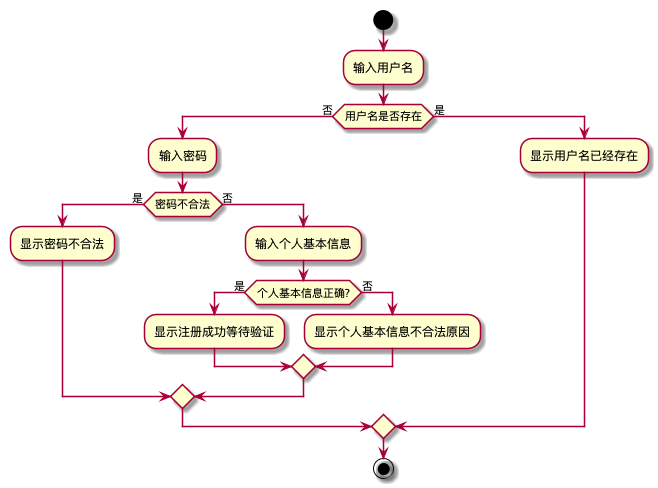
\includegraphics[width=16cm]{report/figure/usecase_v2/uc_enroll.png}
        \caption{用户注册用例-活动图}
        \label{fig:enroll-uml}
        %\end{adjustwidth}
    \end{figure}
    

\begin{enumerate}
    \item \textbf{简要说明}  \\ 本用例描述订购商、微供应商、管理员如何在鲜天下平台进行注册。
    \item \textbf{参与者} \\ 订购商、微供应商、管理员, 以下简称用户。
    \item \textbf{事件流} \\ 相应活动图可见\autoref{fig:enroll-uml}。
    \begin{enumerate} 
        \item \textbf{基本事件流} \\ 本用例开始于用户获取鲜天下平台注册界面。
        \begin{enumerate}
            \item 系统请求用户基本注册信息。
            \item 注册用户输入用户名。
            \item 注册用户输入密码。
            \item 注册用户再次输入密码。
            \item 注册用户输入其他基本信息。
            \begin{enumerate}
                \item 用户名已存在。
                \item 二次密码输入与第一次密码输入不匹配。
                \item 其他信息不合法。
            \end{enumerate}
            \item 用户成功注册并等待验证。
        \end{enumerate}
        \item \textbf{后备事件流}
        \begin{enumerate}
            \item 用户名已存在。
            \begin{enumerate}
                \item 系统显示错误信息 “用户名已存在”。
                \item 返回事件流第一步。
            \end{enumerate}
            \item 二次密码输入与第一次密码输入不匹配。
            \begin{enumerate}
                \item 系统显示错误信息 “两次输入不匹配”。
                \item 返回事件流第二步。
            \end{enumerate}
            \item 其他信息不合法。
            \begin{enumerate}
                \item 系统显示相应错误信息。
                \item 返回事件流第三步。
            \end{enumerate}
        \end{enumerate}
    \end{enumerate}
    \item \textbf{特殊需求} \\ 密码输入框必须以密文方式呈现。
    \item \textbf{前置条件} \\ 用例开始前, 用户需要打开对应的系统注册界面。
    \item \textbf{后置条件} \\ 如果用例成功, 用户信息需要保存在后端数据库中并且用户状态应该设置为待验证状态。
\end{enumerate}

\subsection{登录用例的用例规约}

%\usepackage{changepage}
%\usepackage{rotating}
%\usepackage{float}
%\usepackage[section]{placeins}
%\begin{sidewaystable}[!Htp]
    \begin{figure}[htp]
        %\begin{adjustwidth}{-1.5cm}{-1cm}
        \centering
        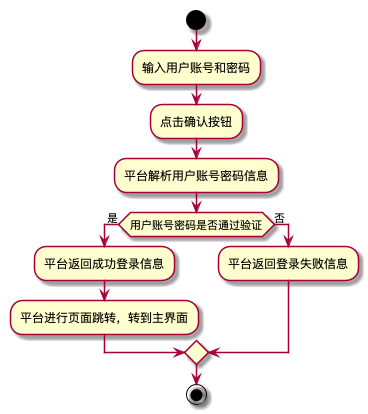
\includegraphics[width=9cm]{report/figure/usecase_v2/uc_login.png}
        \caption{登录用例-活动图}
        \label{fig:logon-uml}
        %\end{adjustwidth}
    \end{figure}
    

\begin{enumerate}
	\item \textbf{简要说明}  \\ 本用例描述订购商、微供应商、管理员如何登录到鲜天下平台。
	\item \textbf{参与者} \\ 订购商、微供应商、管理员, 以下简称用户。
	\item \textbf{事件流} \\ 相应活动图可见\autoref{fig:logon-uml}。
	\begin{enumerate} 
        \item \textbf{基本事件流} \\ 本用例开始于用户希望登录到鲜天下平台,并点击登录按钮。
        \begin{enumerate}
            \item 用户输入用户名和密码。
            \item 用户点击确认按钮。
            \item 平台返回解析结果。
            \begin{enumerate}
                \item 用户账号密码信息通过验证
                \item 用户账号密码信息未通过验证。
            \end{enumerate}
            \item 平台返回成功登录信息。
            \item 平台进行页面跳转,转到主界面。
        \end{enumerate}
        \item \textbf{后备事件流}
        \begin{enumerate}
            \item 用户账号密码信息未通过验证。
            \begin{enumerate}
                \item 系统显示登录失败信息。
                \item 返回事件流第一步。
            \end{enumerate}

        \end{enumerate}
    \end{enumerate}
    \item \textbf{特殊需求} \\ 密码输入框必须以密文方式呈现。
    \item \textbf{前置条件} \\ 用例开始前, 用户需要打开对应的系统登录界面, 且用户处于未登录状态。
    \item \textbf{后置条件} \\ 如果用例成功, 系统状态转换为登录态;若失败, 系统状态不改变。
\end{enumerate}


\subsection{发布母订单用例的用例规约}

\begin{figure}[htp]
        %\begin{adjustwidth}{-1.5cm}{-1cm}
        \centering
        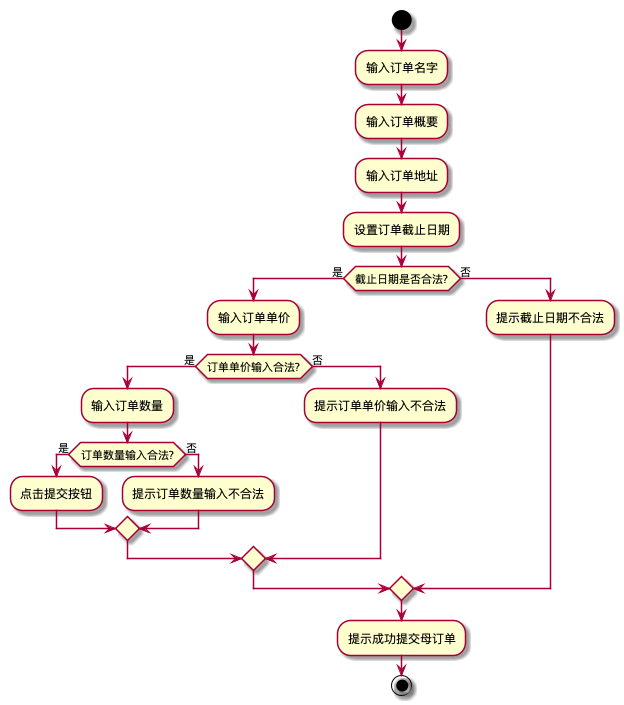
\includegraphics[width=16cm]{figure/usecase_v2/fabu.png}
        \caption{发布母订单-活动图}
        \label{fig:put-mon-order-uml}
        %\end{adjustwidth}
    \end{figure}

\begin{enumerate}
    \item \textbf{简要说明}  \\ 本用例允许采购商向"鲜天下"平台提交母订单。在完成了登录后,采购商可以进入"鲜天下"平台发布母订单界面,然后向"鲜天下"平台提交生成母订单请求。
    \item \textbf{参与者} \\ 采购商。
    \item \textbf{事件流} \\ 相应活动图可见\autoref{fig:put-mon-order-uml}。
    \begin{enumerate} 
        \item \textbf{基本事件流} \\ 本用例开始于供应商登录到"鲜天下"平台,并点击发起母订单。
        \begin{enumerate}
            \item 输入订单名字 
            \item 输入订单概要 
            \item 输入订单地址 
            \item 选择订单截止日期 
            \item 平台检测截止日期是否合法 
            \begin{enumerate}
                \item 截止日期是否是过去时间
            \end{enumerate}

            \item 用户输入订单单价 
            \begin{enumerate}
                \item 订单单价是非数字字符串
                \item 订单单价是负数
            \end{enumerate}
            %tips:不知道还要加什么信息

            \item 用户输入订单数量 
            \begin{enumerate}
                \item 订单数量是非数字字符串
                \item 订单数量是负数
            \end{enumerate}

            \item 用户点击提交按钮
            \item 平台提示成功提交的信息

        \end{enumerate}

        \item \textbf{后备事件流}
        \begin{enumerate}
            \item 截止日期不合法
            \begin{enumerate}
                \item 平台提示截止日期不合法
                \item 返回第四步
            \end{enumerate}

            \item 订单单价输入不合法
            \begin{enumerate}
                \item 平台提示订单单价不合法
                \item 返回第五步
            \end{enumerate}

            \item 订单数量输入不合法
            \begin{enumerate}
                \item 平台提示订单数量输入不合法
                \item 返回第六步
            \end{enumerate}
        \end{enumerate}
    \end{enumerate}
    \item \textbf{特殊需求} \\ 截止日期应该是一个有内容待选界面的输入。
    \item \textbf{前置条件} \\ 用例开始前, 供应商用户需要处于已登录状态下, 并进入于发布母订单界面。
    \item \textbf{后置条件} \\ 在数据库中暂存母订单信息,状态为"待审核"状态。经过管理员的进一步审核后,如果订单通过管理员的审核,则将订单状态从"待审核状态"改为"待执行"状态,使得订单能够被分派出去成为"执行中"状态;如果订单没有通过审核,在审核后将订单状态改为"未通过审核"状态,并在一个月后将订单丢弃。人工面谈后交付定金),订单状态均切换为待完成态。
\end{enumerate}



\subsection{查看母订单用例的用例规约}
\begin{figure}[htp]
    %\begin{adjustwidth}{-1.5cm}{-1cm}
    \centering
    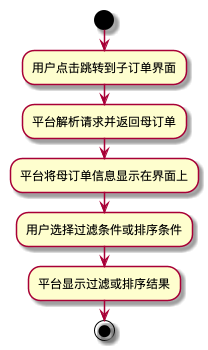
\includegraphics[width=5cm]{figure/usecase_v2/query_mainOrder.png}
    \caption{商查看母订单用例-活动图}
    \label{fig:uc_order_query-uml}
    %\end{adjustwidth}
\end{figure}

\begin{enumerate}
    \item \textbf{简要说明}  \\ 本用例允许用户查看所有母订单信息,同时也允许。
    \item \textbf{参与者} \\ 采购商、管理员、微供应商,统称用户。
    \item \textbf{事件流} \\ 相应活动图可见\autoref{fig:uc_order_query-uml}。
    \begin{enumerate} 
        \item \textbf{基本事件流} \\ 本用例开始于用户已经登录进入平台。
        \begin{enumerate}
            \item 用户点击跳转到母订单界面的按钮。

            \item "鲜天下"平台解析请求并获取所有母订单信息。

            \item "鲜天下"平台将所有母订单信息显示在界面上。

            \item 用户选择过滤条件或排序条件。
            
            \item "鲜天下"平台将过滤或排序结果显示给用户。

        \end{enumerate}
        \item \textbf{后备事件流}  \\ 无。
        
    \end{enumerate}
    \item \textbf{特殊需求} \\ 无。
    \item \textbf{前置条件} \\ 本用例开始前用户已经登录进入"鲜天下"平台。
    \item \textbf{后置条件} \\ 本用例不对数据库作任何修改。
\end{enumerate}



\subsection{查看子订单用例的用例规约}
\begin{figure}[htp]
    %\begin{adjustwidth}{-1.5cm}{-1cm}
    \centering
    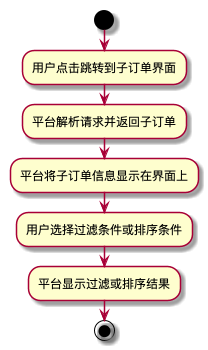
\includegraphics[width=5cm]{figure/usecase_v2/query_subOrder.png}
    \caption{查看子订单用例-活动图}
    \label{fig:uc_suborder_query}
    %\end{adjustwidth}
\end{figure}

\begin{enumerate}
    \item \textbf{简要说明}  \\ 本用例允许用户查看所有子订单信息。
    \item \textbf{参与者} \\ 采购商、微供应商、管理员,以下称用户。
    \item \textbf{事件流} \\ 相应活动图可见\autoref{fig:uc_suborder_query}。
    \begin{enumerate} 
        \item \textbf{基本事件流} \\ 本用例开始于用户已经登录进入"鲜天下"平台。
        \begin{enumerate}
            \item 用户点击跳转到子订单界面的按钮。

            \item "鲜天下"平台解析请求并获取所有子订单信息。

            \item "鲜天下"平台将所有子订单信息显示在界面上。

            \item 用户选择过滤条件或排序条件。
            
            \item "鲜天下"平台将过滤或排序结果显示给用户。

        \end{enumerate}

        \item \textbf{后备事件流}  \\ 无。
        
    \end{enumerate}
    \item \textbf{特殊需求} \\ 无。
    \item \textbf{前置条件} \\ 本用例开始前用户已经登录进入"鲜天下"平台。
    \item \textbf{后置条件} \\ 本用例不对数据库作任何修改。
\end{enumerate}




\subsection{加入母订单用例的用例规约}
\begin{figure}[htp]
    %\begin{adjustwidth}{-1.5cm}{-1cm}
    \centering
    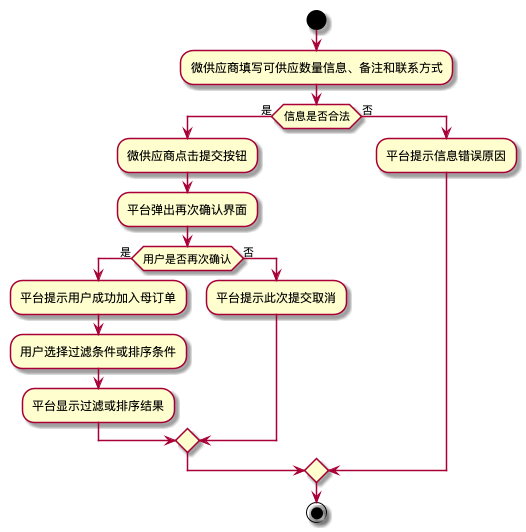
\includegraphics[width=14cm]{figure/usecase_v2/join.png}
    \caption{加入母订单用例-活动图}
    \label{fig:uc_order_commit}
    %\end{adjustwidth}
\end{figure}

\begin{enumerate}
    \item \textbf{简要说明}  \\ 本用例允许微供应商在"鲜天下"平台以类似众筹的方式加入还未完成母订单。
    \item \textbf{参与者} \\ 微供应商。
    \item \textbf{事件流} \\ 相应活动图可见\autoref{fig:uc_order_commit}。
    \begin{enumerate} 
        \item \textbf{基本事件流} \\ 本用例开始于供应商进入母订单页面,并点击加入母订单。
        \begin{enumerate}
            \item 微供应商填写可供应数量、备注和联系方式
            %tips:不知道还要加什么信息

            \item 平台检查微供应商的输入信息是否合法
            \begin{enumerate}
                \item 微供应商填写数量超过母订单当前需要的数量
                \item 微供应商填写的联系方式不合法
            \end{enumerate}

            \item 用户点击提交按钮。

            \item 平台弹出再次确认界面
            \begin{enumerate}
                \item 用户点击确认按钮
                \item 用户点击否认按钮
            \end{enumerate}

            \item 平台提示用户成功加入母订单
            

        \end{enumerate}
        \item \textbf{后备事件流}
        \begin{enumerate}
            \item 微供应商填写数量超过母订单当前需要的数量
            \begin{enumerate}
                \item 平台提醒微供应商当前数量不合法
            \end{enumerate}

            \item 微供应商填写的联系方式不合法
            \begin{enumerate}
                \item 平台提醒微供应商的联系方式输入不合法
            \end{enumerate}

            \item 用户点击否认按钮
            \begin{enumerate}
                \item 返回第二步
            \end{enumerate}
        \end{enumerate}
    \end{enumerate}
    \item \textbf{特殊需求} \\ 无。
    \item \textbf{前置条件} \\ 用例开始前, 供应商用户需要处于已登录状态下, 处于有生成母订单的界面。
    \item \textbf{后置条件} \\ 如果用户成功加入母订单后,要在后端数据库形成相应的子订单信息,并修改母订单信息。

\end{enumerate}

\subsection{审核新用户用例的用例规约}

\begin{figure}[htp]
    %\begin{adjustwidth}{-1.5cm}{-1cm}
    \centering
    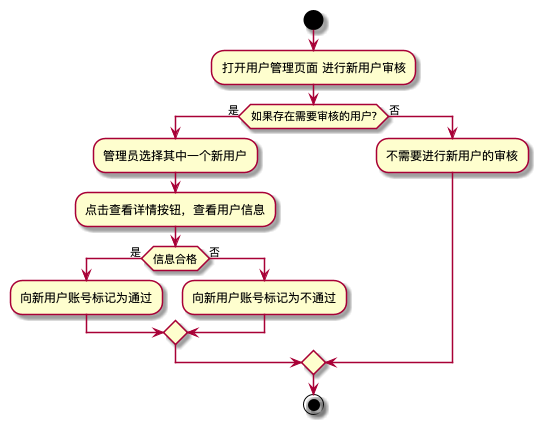
\includegraphics[width=14cm]{report/figure/usecase_v2/1_uc_admin_check_user.png}
    \caption{审核新用户用例-活动图}
    \label{fig:1_uc_admin_check_user}
    %\end{adjustwidth}
\end{figure}


\begin{enumerate}
	\item \textbf{简要说明}  \\ 本用例描述管理员如何审核新用户的资质。
	\item \textbf{参与者} \\ 管理员。
	\item \textbf{事件流} \\ 相应活动图可见\autoref{fig:1_uc_admin_check_user}。
	\begin{enumerate} 
        \item \textbf{基本事件流} \\ 本用例开始于处于登录态的管理员对在“鲜天下”平台注册且未被审核的新用户进行审核。
        \begin{enumerate}
            \item 管理员打开用户管理页面
            \item 平台向管理员展示当前目前系统中的用户列表。
            \item 管理员选择其中一个新用户,并点击“查看详情”按钮。
            \item 平台显示该新用户的详细信息。
            \begin{enumerate}
                \item 系统将会以表单的形式,向管理员展示新用户为了注册而填写的表单,同时会有滑块,由管理员选择是否审核通过。
            \end{enumerate}
            \item 由管理员决定该审核是否通过。
            \begin{enumerate}
                \item 管理员将滑块滑向右边表示通过。
                \item 管理员将滑块滑向左边表示不通过。
            \end{enumerate}
            \item 用户列表上将会展示用户账户当前的新状态。
        \end{enumerate}
        \item \textbf{后备事件流} \\
        \begin{enumerate}
            \item 管理员否决此次审核。
            \begin{enumerate}
                \item 滑块滑向左边后,返回到用户列表。
            \end{enumerate}
            \item 没有需要审核的新用户。
            \begin{enumerate}
                \item 管理员无须进行操作。
            \end{enumerate}
        \end{enumerate}
    \end{enumerate}
    \item \textbf{特殊需求} 
    \begin{enumerate}
        \item 用户管理页面的用户列表中,用户状态一列将会展示该用户的激活状态。
        \item 设置激活状态的滑块滑向左边表示未审核通过,右边表示审核通过。
    \end{enumerate}
    \item \textbf{前置条件} \\ 用例开始前, 管理员需要处于已登录状态下, 并打开用户管理界面。
    \item \textbf{后置条件} \\ 如果某新用户审核通过,与该新用户相关的状态将被更新到数据库中。
\end{enumerate}



\subsection{修改用户信息用例的用例规约}

\begin{figure}[htp]
    %\begin{adjustwidth}{-1.5cm}{-1cm}
    \centering
    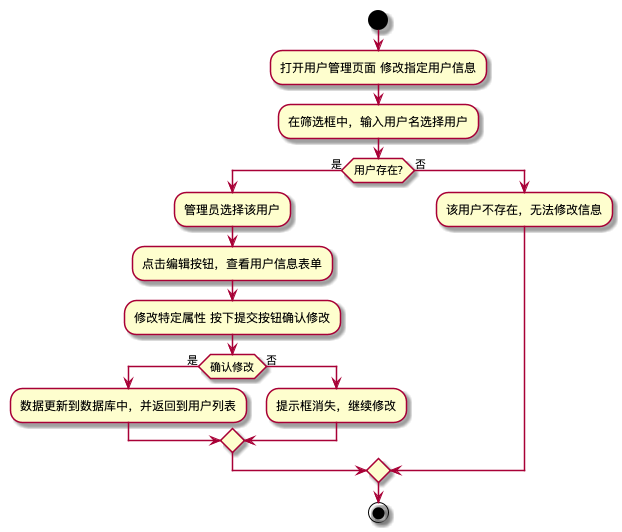
\includegraphics[width=16cm]{report/figure/usecase_v2/2_uc_admin_edit_user_info.png}
    \caption{修改用户信息用例-活动图}
    \label{fig:2_uc_admin_edit_user_info}
    %\end{adjustwidth}
\end{figure}


\begin{enumerate}
	\item \textbf{简要说明}  \\ 本用例描述管理员如何对系统中的所有用户的信息进行修改。
	\item \textbf{参与者} \\ 管理员。
	\item \textbf{事件流} \\ 相应活动图可见\autoref{fig:2_uc_admin_edit_user_info}。
	\begin{enumerate} 
        \item \textbf{基本事件流} \\ 本用例开始于处于登录态的管理员对在“鲜天下”平台注册的新用户的信息进行修改。
        \begin{enumerate}
            \item 管理员打开用户管理页面
            \item 平台向管理员展示当前目前系统中的用户列表。
            \item 管理员选择其中一个新用户,按下“编辑”按钮。
            \begin{enumerate}
                \item 系统将会以表单的形式,向管理员展示用户现有信息,包含用户名,手机号码,账户余额,用户类型,用户状态。
            \end{enumerate}
            \item 管理员在需要修改的属性的输入框中输入修改后的信息。
            \item 管理员按下“提交”按钮确认提交
            \item 平台弹出一个提示框确认管理员的提交。
            \begin{enumerate}
                \item 按下确认按钮。
                \item 按下取消按钮。
            \end{enumerate}
            \item 则当前的修改信息确认更新,并返回到用户列表页面中,用户列表将会展示用户最新的信息。
        \end{enumerate}
        \item \textbf{后备事件流}
        \begin{enumerate}
            \item 在确认管理员修改操作的提示框中,管理员按下取消按钮。
            \begin{enumerate}
                \item 则提示框消失,管理员可继续编辑,并尝试再次提交。
            \end{enumerate}
        \end{enumerate}
    \end{enumerate}
    \item \textbf{特殊需求}
    \begin{enumerate}
        \item 用户列表中,每一个用户的操作一列都将会有编辑按钮,管理员可通过该按钮编辑指定用户信息。
        \item 在用户信息的编辑页面中,用户名不可修改,其他属性均可修改。
    \end{enumerate}
    \item \textbf{前置条件} \\ 用例开始前, 管理员需要处于已登录状态下, 并打开用户管理界面。
    \item \textbf{后置条件} \\ 如果某新用户信息确认修改,与该新用户相关的修改信息将被更新到数据库中。
\end{enumerate}



% \subsection{删除特定用户用例的用例规约}

% \begin{figure}[htp]
%     %\begin{adjustwidth}{-1.5cm}{-1cm}
%     \centering
%     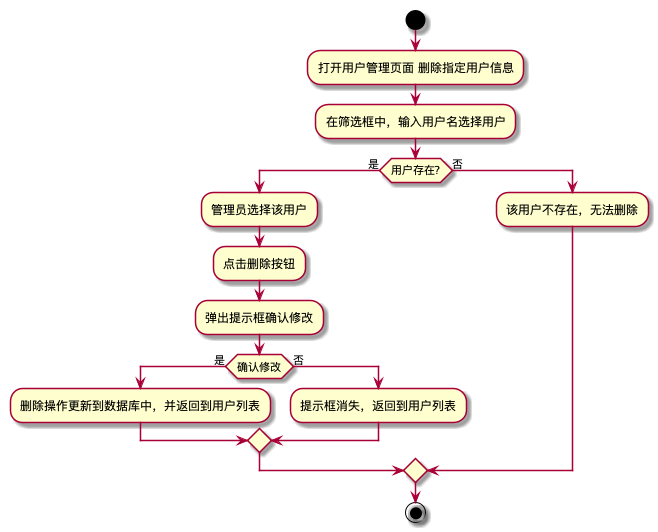
\includegraphics[width=16cm]{report/figure/usecase_v2/3_uc_admin_delete_user.png}
%     \caption{删除特定用户用例-活动图}
%     \label{fig:3_uc_admin_delete_user}
%     %\end{adjustwidth}
% \end{figure}


% \begin{enumerate}
% 	\item \textbf{简要说明}  \\ 本用例描述管理员如何删除特定的用户。
% 	\item \textbf{参与者} \\ 管理员。
% 	\item \textbf{事件流} \\ 相应活动图可见\autoref{fig:3_uc_admin_delete_user}。
% 	\begin{enumerate} 
%         \item \textbf{基本事件流} \\ 本用例开始于处于登录态的管理员需要删除在“鲜天下”平台注册的用户。
%         \begin{enumerate}
%             \item 管理员打开用户管理页面。
%             \item 平台向向理员展示目前系统中的用户列表。
%             \item 管理员选择其中一个新用户,按下删除按钮。
%             \item 平台会弹出一个提示框确认管理员的删除。
%             \begin{enumerate}
%                 \item 按下确认按钮。
%                 \item 按下取消按钮。
%             \end{enumerate}
%             \item 当前的删除操作生效,并返回到用户列表页面中。
%         \end{enumerate}
%         \item \textbf{后备事件流}
%         \begin{enumerate}
%             \item 在平台弹出的确认提示框中,管理员按下取消按钮。
%             \begin{enumerate}
%                 \item 提示框消失,管理员的删除操作失效。
%             \end{enumerate}
%         \end{enumerate}
%     \end{enumerate}
%     \item \textbf{特殊需求}
%     \begin{enumerate}
%         \item 用户列表中,每一个用户的操作一列都将会有红色删除按钮,管理员可通过该按钮删除指定用户。
%     \end{enumerate}
%     \item \textbf{前置条件} \\ 用例开始前, 管理员需要处于已登录状态下, 并打开用户管理界面。
%     \item \textbf{后置条件} \\ 如果某新用户删除操作经过确认,删除操作将导致该用户信息从数据库中删除。
% \end{enumerate}


\subsection{母订单管理用例的用例规约}

\begin{figure}[htp]
    %\begin{adjustwidth}{-1.5cm}{-1cm}
    \centering
    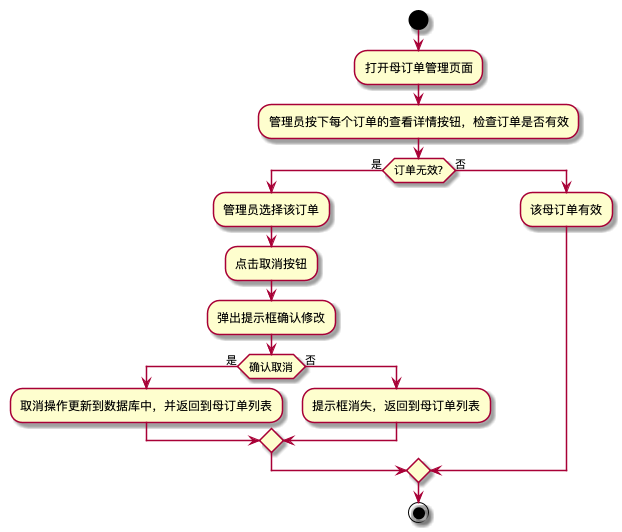
\includegraphics[width=16cm]{report/figure/usecase_v2/4_uc_admin_manage_mainOrder.png}
    \caption{母订单管理用例-活动图}
    \label{fig:4_uc_admin_manage_mainOrder}
    %\end{adjustwidth}
\end{figure}


\begin{enumerate}
	\item \textbf{简要说明}  \\ 本用例描述管理员如何审核并取消特定的母订单。
	\item \textbf{参与者} \\ 管理员。
	\item \textbf{事件流} \\ 相应活动图可见\autoref{fig:4_uc_admin_manage_mainOrder}。
	\begin{enumerate} 
        \item \textbf{基本事件流} \\ 本用例开始于处于登录态的管理员需要对在“鲜天下”平台发布的母订单进行审核,并取消无效母订单。
        \begin{enumerate}
            \item 管理员打开母订单管理页面。
            \item 平台向管理员展示当前目前系统中的母订单列表。
            \item 管理员选择其中一个母订单,按下查看详情按钮。
            \item 平台会向管理员展示该订单的所有信息。
            \begin{enumerate}
                \item 母订单的信息包括地址,创建日期,截止日期,订单名称,订单内容,货物单价,货物数量,订单总价,以及联系人手机号码。
            \end{enumerate}
            \item 管理员对该母订单进行审核。
            \begin{enumerate}
                \item 管理员认为母订单无效。
                \item 管理员认为母订单有效。
            \end{enumerate}
            \item 管理员按下取消按钮,
            \item 平台弹出一个提示框确认管理员的取消操作。
            \begin{enumerate}
                \item 按下确认按钮。
                \item 按下取消按钮。
            \end{enumerate}
            \item 当前的取消操作生效,并返回到母订单列表页面中。
        \end{enumerate}
        \item \textbf{后备事件流}
        \begin{enumerate}
            \item 管理员认为母订单有效。
            \begin{enumerate}
                \item 管理员无需操作,返回母订单列表。
            \end{enumerate}
            \item 在平台弹出的取消操作确认提示框中,管理员按下取消按钮。
            \begin{enumerate}
                \item 提示框消失,取消操作失效,返回到母订单列表页面中。
            \end{enumerate}
        \end{enumerate}
    \end{enumerate}
    \item \textbf{特殊需求}
    \begin{enumerate}
        \item 母订单列表中,每一个母订单都将会有查看详情按钮,管理员可通过该按钮查看指定母订单的详细信息。
        \item 母订单列表中,每一个母订单都将会有取消按钮,管理员可通过该按钮取消指定的母订单。
    \end{enumerate}
    \item \textbf{前置条件} \\ 用例开始前, 管理员需要处于已登录状态下, 并打开母订单管理界面。
    \item \textbf{后置条件} \\ 如果某母订单的取消操作经过确认,取消操作将会让指定母订单的状态从“正在进行中”变为“已取消”,并将相应信息更新到数据库中。
\end{enumerate}



\subsection{子订单管理用例的用例规约}

\begin{figure}[htp]
    %\begin{adjustwidth}{-1.5cm}{-1cm}
    \centering
    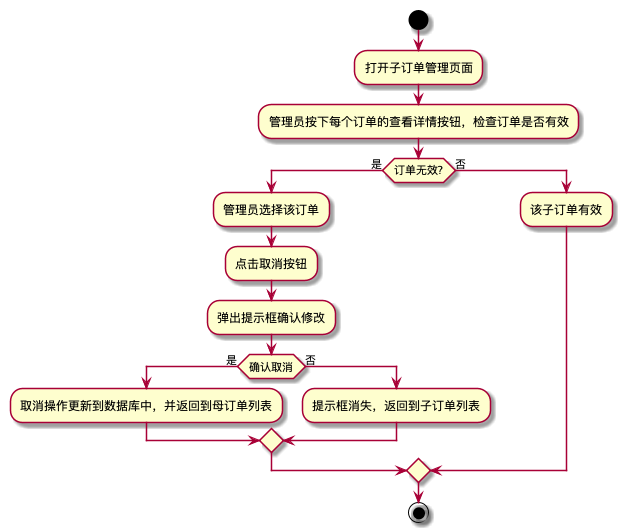
\includegraphics[width=16cm]{report/figure/usecase_v2/5_uc_admin_manage_subOrder.png}
    \caption{子订单管理用例-活动图}
    \label{fig:5_uc_admin_manage_subOrder}
    %\end{adjustwidth}
\end{figure}


\begin{enumerate}
	\item \textbf{简要说明}  \\ 本用例描述管理员如何审核并取消特定的子订单。
	\item \textbf{参与者} \\ 管理员。
	\item \textbf{事件流} \\ 相应活动图可见\autoref{fig:5_uc_admin_manage_subOrder}。
	\begin{enumerate} 
        \item \textbf{基本事件流} \\ 本用例开始于处于登录态的管理员需要对在“鲜天下”平台发布的子订单进行审核,并取消无效子订单。
        \begin{enumerate}
            \item 管理员打开子订单管理页面。
            \item 平台向管理员展示当前目前系统中的子订单列表。
            \item 管理员选择其中一个子订单,按下查看详情按钮。
            \item 平台会向管理员展示该订单的所有信息。
            \begin{enumerate}
                \item 子订单的信息包括创建日期,货物数量,联系人手机号码以及备注。
            \end{enumerate}
            \item 管理员对该子订单进行审核。
            \begin{enumerate}
                \item 管理员认为子订单无效。
                \item 管理员认为子订单有效。
            \end{enumerate}
            \item 管理员按下取消按钮,
            \item 平台弹出一个提示框确认管理员的取消操作。
            \begin{enumerate}
                \item 按下确认按钮。
                \item 按下取消按钮。
            \end{enumerate}
            \item 当前的取消操作生效,并返回到子订单列表页面中。
        \end{enumerate}
        \item \textbf{后备事件流}
        \begin{enumerate}
            \item 管理员认为子订单有效。
            \begin{enumerate}
                \item 管理员无需操作,返回母订单列表。
            \end{enumerate}
            \item 在平台弹出的取消操作确认提示框中,管理员按下取消按钮。
            \begin{enumerate}
                \item 提示框消失,取消操作失效,返回到子订单列表页面中。
            \end{enumerate}
        \end{enumerate}
    \end{enumerate}
    \item \textbf{特殊需求}
    \begin{enumerate}
        \item 子订单列表中,每一个子订单都将会有查看详情按钮,管理员可通过该按钮查看指定子订单的详细信息。
        \item 子订单列表中,每一个子订单都将会有取消按钮,管理员可通过该按钮取消指定的子订单。
    \end{enumerate}
    \item \textbf{前置条件} \\ 用例开始前, 管理员需要处于已登录状态下, 并打开子订单管理界面。
    \item \textbf{后置条件} \\ 如果某子订单的取消操作经过确认,取消操作将会让指定子订单的状态从“正在进行中”变为“已取消”,并将相应信息更新到数据库中。
\end{enumerate}

\subsection{余额提现用例的用例规约}
\begin{figure}[htp]
    %\begin{adjustwidth}{-1.5cm}{-1cm}
    \centering
    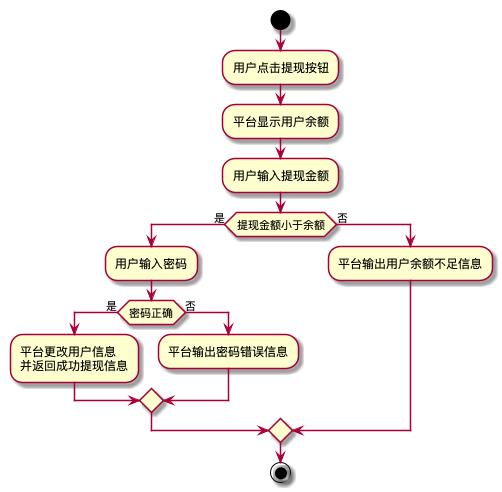
\includegraphics[width=12cm]{report/figure/usecase_v2/withdraw.png}
    \caption{余额提现用例-活动图}
    \label{fig:withdraw}
    %\end{adjustwidth}
\end{figure}


\begin{enumerate}
	\item \textbf{简要说明}  \\ 本用例描述微供应商和采购商如何从个人钱包中提现。
	\item \textbf{参与者} \\ 管理员。
	\item \textbf{事件流} \\ 相应活动图可见\autoref{fig:withdraw}。
	\begin{enumerate} 
        \item \textbf{基本事件流} \\ 本用例开始于处于登录态的微供应商或采购商(以下称用户)希望进行提现操作。
        \begin{enumerate}
            \item 用户点击提现按钮。
            \item 平台向用户展示用户余额。
            \item 用户输入充值金额。
            \begin{enumerate}
                \item 提现金额小于余额
                \item 提现金额大于余额
            \end{enumerate}
            \item 用户输入密码。
            \begin{enumerate}
                \item 密码正确。
                \item 密码错误。
            \end{enumerate}
            \item 平台更改用户余额并返回成功提现信息。
        \end{enumerate}
        \item \textbf{后备事件流}
            \begin{enumerate}
                \item 提现金额大于余额
            \begin{enumerate}
                \item 提示“提现金额大于余额”,并返回第三步。
            \end{enumerate}
            
            \item 密码错误。
            \begin{enumerate}
                \item 提示用户密码错误,并返回第四步。
            \end{enumerate}
            \end{enumerate}
    \end{enumerate}
    \item \textbf{特殊需求}
    \begin{enumerate}
        \item 用户输入的密码已密文形式呈现。
        \item 提现事务必须是原子操作,要么将流程图执行完,要么都不执行。
    \end{enumerate}
    \item \textbf{前置条件} \\ 用例开始前, 微供应商和采购商需要处于已登录状态下。
    \item \textbf{后置条件} \\ 修改后的个人钱包信息被稳定的储存在数据库中。 
\end{enumerate}


\subsection{钱包充值用例的用例规约}
\begin{figure}[htp]
    %\begin{adjustwidth}{-1.5cm}{-1cm}
    \centering
    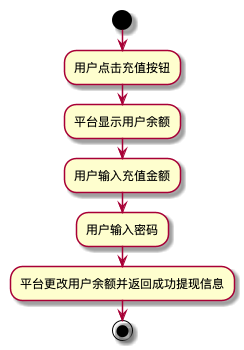
\includegraphics[width=7cm]{report/figure/usecase_v2/topup.png}
    \caption{钱包充值用例用例-活动图}
    \label{fig:topup}
    %\end{adjustwidth}
\end{figure}


\begin{enumerate}
	\item \textbf{简要说明}  \\ 本用例描述微供应商和采购商如何向个人钱包中充值。
	\item \textbf{参与者} \\ 微供应商和采购商。
	\item \textbf{事件流} \\ 相应活动图可见\autoref{fig:topup}。
	\begin{enumerate} 
        \item \textbf{基本事件流} \\ 本用例开始于处于登录态的微供应商或采购商(以下称用户)希望进行充值操作。
        \begin{enumerate}
            \item 用户点击充值按钮。
            \item 平台向用户展示用户余额。
            \item 用户输入充值金额。
            \item 用户输入密码。
            \item 平台更改用户余额并返回成功充值信息。
        \end{enumerate}
        \item \textbf{后备事件流} \\
            无。
    \end{enumerate}
    \item \textbf{特殊需求}
    \begin{enumerate}
        \item 用户输入的密码已密文形式呈现。
        \item 充值事务必须是原子操作,要么将流程图执行完,要么都不执行。
    \end{enumerate}
    \item \textbf{前置条件} \\ 用例开始前, 微供应商和采购商需要处于已登录状态下。
    \item \textbf{后置条件} \\ 修改后的个人钱包信息被稳定的储存在数据库中。 
\end{enumerate}


\subsection{审核新用户用例的用例规约}
\begin{figure}[htp]
    %\begin{adjustwidth}{-1.5cm}{-1cm}
    \centering
    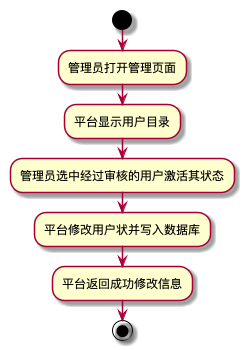
\includegraphics[width=7cm]{report/figure/usecase_v2/activate.png}
    \caption{审核新用户用例-活动图}
    \label{fig:activate}
    %\end{adjustwidth}
\end{figure}


\begin{enumerate}
	\item \textbf{简要说明}  \\ 本用例描述管理员如何对系统中的经过审核的新用户进行状态激活。
	\item \textbf{参与者} \\ 管理员。
	\item \textbf{事件流} \\ 相应活动图可见\autoref{fig:activate}。
	\begin{enumerate} 
        \item \textbf{基本事件流} \\ 本用例开始于处于登录态的管理员对在“鲜天下”平台注册的新用户的信息进行审核。
        \begin{enumerate}
            \item 管理员打开用户管理页面。
            \item 平台向管理员展示当前目前系统中的用户列表。
            \item 管理员选择其中一个经过人工审核的新用户,点击其状态栏进行状态切换。
            \item 平台修改用户状态并写入数据库。
            \item 平台返回成功修改信息。
        \end{enumerate}
        \item \textbf{后备事件流}
            无。
    \end{enumerate}
    \item \textbf{特殊需求}
    \begin{enumerate}
        \item 用户的状态要表示成两状态可切换状态栏。
    \end{enumerate}
    \item \textbf{前置条件} \\ 用例开始前, 管理员需要处于已登录状态下。
    \item \textbf{后置条件} \\ 如果用新用户的状态被管理员修改
\end{enumerate}


%\usepackage{changepage}
%\usepackage{rotating}
%\usepackage{float}
%\usepackage[section]{placeins}
%\begin{sidewaystable}[!Htp]


\section{"鲜天下"实现补充规约}

% TODO: 等其他部分写完了,再回来继续水水这里

    补充规约列出了不便于在用例模型的用例中获取的系统需求。补充规约用例模型一起记录关于系统的一整套需求。


\subsection{范围}
    \begin{enumerate}

        \item 本补充规约适用于"鲜天下"系统,将要由学习面向对象软件分析与设计的学生开发。
        \item 本规约除定义了在许多用例中所共有的功能性需求以外,还定义了系统的非功能性需求,例如:可靠性、可用性、性能和可支持性等。

    \end{enumerate}

\subsection{可靠性}

    "鲜天下"交易平台应该在每周七天,每天二十四小时内都应是可以使用的。宕机的时间应少于 5\%。配备有2名维护人员,轮流提供维护服务。


\subsection{性能}
    \begin{enumerate}
        \item 通过CDN服务使得服务器的平均响应时间不能超过1秒。
    \end{enumerate}

\subsection{安全性}
    \begin{enumerate}
        \item 通过后端用户输入过滤来防范XSS攻击。
        \item 服务端配置完善的跨域规则,同时利用后端框架提供的CSRF\_TOKEN防范CSRF攻击。
        \item 全站采用HTTPS、密码等不对称加密方式加密后传输防范中间人攻击。
        \item 采用后端框架提供的参数化查询来避免SQL注入攻击。
    \end{enumerate}

\newpage
\section{术语表}

\begin{table}[h] %voc table result
 \begin{adjustwidth}{-1cm}{-1cm}
	\centering
        \label{tab:glossary}
        \caption{“鲜天下”-术语表}
		\begin{tabular}{*{5}{c}}
			\toprule
	 		编号 & 术语 & 含义\\
            \midrule
            1 & 微供应商 & 生产虾的微小供应商, 为平台上实际货物的生产者 \\
            2 & 订购商 & 购买虾的订购商, 为平台上实际货物的购买者 \\
            3 & 管理员 & 管理订单和用户,为平台上所有订单和用户的管理者\\
            4 & 平台 & 连接微供应商和订购商的桥梁, 负责订单派发, 资金分派, 物流等功能\\
			\bottomrule
		\end{tabular}
    \end{adjustwidth}
\end{table}
